\aula{01b}{20}{agosto}{2026}

\chapter*{Exercício}

\begin{enumerate}
    \item Considerando a planta de forma estrutural apresentada, pede-se:

    \begin{figure}[H]
        \centering
        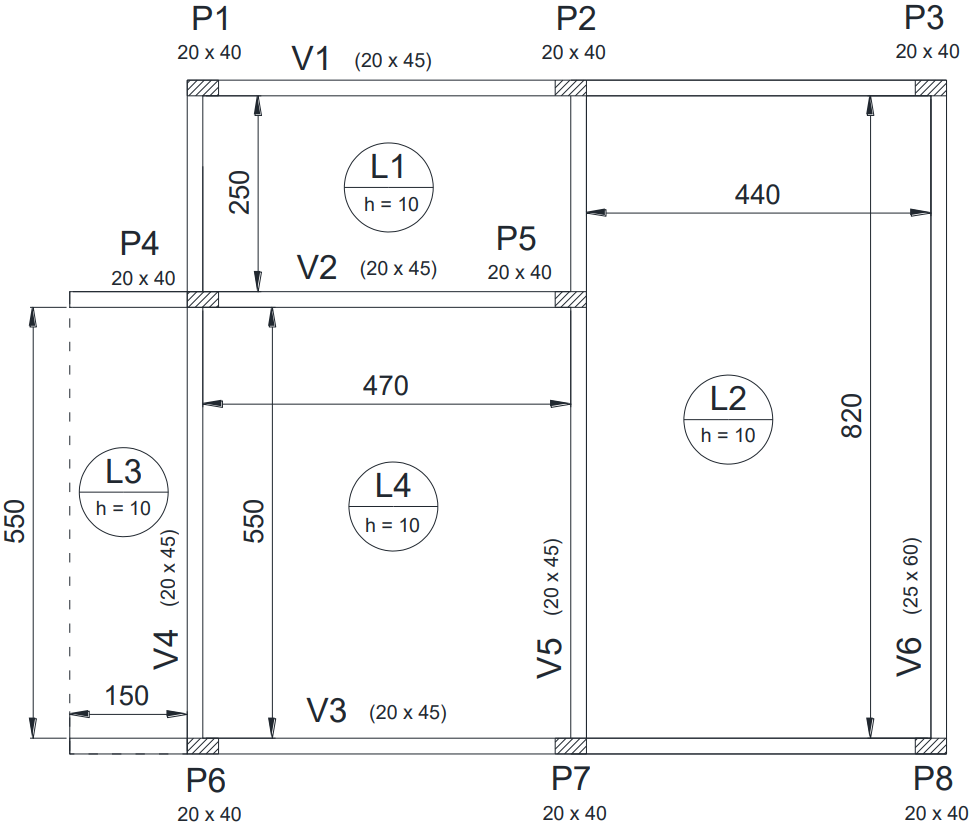
\includegraphics[width=1\linewidth]{assets/images/forma-pavimento-tipo.png}
        \caption{Forma pavimento tipo.}
        \label{fig:forma-pavimento-tipo}
    \end{figure}
    
    \begin{itemize}
        \item classificar as lajes em armadura me uma ou duas direções;
        \item indicar a vinculação de cada uma das lajes;
        \item considerando carregamento permanente $g=3,5 \ kN/m^2$ (peso próprio da laje + peso próprio do piso e revestimentos) e carregamento variável normal $q=3 \ kN/m^2$ (edifícios comerciais), calcular as reações de apoio das lajes.
        \item considerando carregamento permanente $g=3,5 \ kN/m^2$ e carregamento variável normal $q=3\ kN/m^2$, calcular e compatibilizar os momentos atuando nas lajes.
    \end{itemize}
\end{enumerate}

\begin{resposta}
    \begin{enumerate}
        \item Determinação dos vãos efetivos e classificação

        \begin{observacao}
            \begin{math}
                l_x \ \text{menor dimensão} \newline
                l_x \ \text{maior dimensão}
            \end{math}
        \end{observacao}

        \begin{observacao}
            \begin{math}
            b_{w_0} \ \text{zero é a indicação da viga}
            \end{math}
        \end{observacao}

        \begin{observacao}
            \begin{math}
                \lambda \leq 2 \ \text{armada em duas direções} \newline
                \lambda > 2 \ \text{armada em uma direção}
            \end{math}
        \end{observacao}

        \fbox{L1}

        \begin{figure}[H]
    \centering
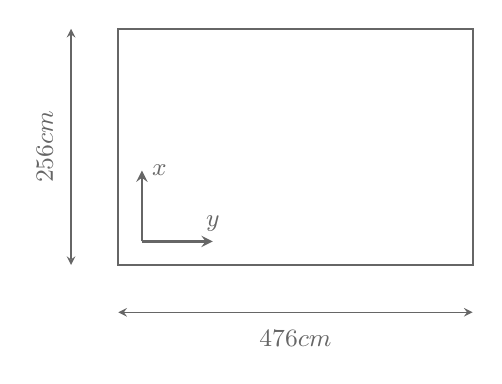
\begin{tikzpicture}[
    scale=1.5,
    cota/.style={<->, >=stealth, thin, gray!80!black},  % Estilo das linhas de cota
    retangulo/.style={draw=gray!80!black, thick},% Estilo do retângulo
    eixo/.style={->, >=stealth, thick, gray!80!black}   % Estilo dos eixos x e y
]

    % 1. Coordenadas do retângulo
    \coordinate (A) at (0, 0);
    \coordinate (B) at (3, 0);
    \coordinate (C) at (3, 2);
    \coordinate (D) at (0, 2);

    % 2. Desenho do Retângulo
    \draw[retangulo] (A) rectangle (C);

    % 3. Eixos de Coordenadas x e y (Origem no canto inferior esquerdo, dentro do retângulo)
    \draw[eixo] (0.2, 0.2) -- (0.8, 0.2) node[above, font=\small\bfseries] {$y$};
    \draw[eixo] (0.2, 0.2) -- (0.2, 0.8) node[right, font=\small\bfseries] {$x$};

    % --- COTA HORIZONTAL (Texto abaixo da linha) ---
    \def\offsetH{0.4}
    \draw[cota] (0, -\offsetH) -- (3, -\offsetH) 
        node[midway, below=3pt, font=\small] {$476\text{ cm}$};

    % --- COTA VERTICAL (Texto à esquerda da linha) ---
    \def\offsetV{0.4}
    \draw[cota] (-\offsetV, 0) -- (-\offsetV, 2) 
        node[midway, left=3pt, font=\small, rotate=90, anchor=south] {$256 \text{ cm}$};

\end{tikzpicture}
    %\caption{Caption}
    %\label{fig:placeholder}
\end{figure}

        \begin{enumerate}
        
        \begin{multicols}{2}
            \item Direção horizontal

            $l_0= 470 \ cm$

            $a_1 \leq \begin{cases}
                \frac{b_{w_4}}{2} = \frac{20}{2}=10 \ cm \\
                0,3h = 0,3 \times 10 = 3 \ cm
            \end{cases}$

            $a_2 \leq \begin{cases}
                \frac{b_{w_5}}{2} = 10 \ cm \\
                0,3 h = 3 \ cm
            \end{cases}$

            $l_{ef}= l_0 +a_1+a_2 = 476 \ cm$
            
            \item Direção vertical

            $l_0= 000 \ cm$

            $a_1 \leq \begin{cases}
                \frac{b_{w_1}}{2} = 10 \ cm \\
                0,3h = 3 \ cm
            \end{cases}$

            $a_2 \leq \begin{cases}
                \frac{b_{w_2}}{2} = 10 \ cm \\
                0,3 h = 3 \ cm
            \end{cases}$

            $l_{ef}= l_0 +a_1+a_2 = 256 \ cm$
        \end{multicols}

            $\lambda = \frac{l_y}{l_x} = \frac{476}{256} \approx 1,86 \leq 2 \to$ armada em duas direções
            
        \end{enumerate}

        \fbox{L2}

        \begin{figure}[H]
    \centering
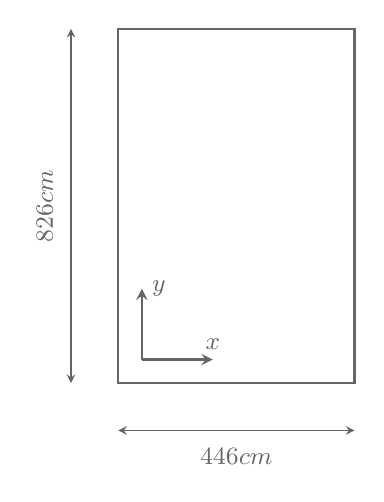
\begin{tikzpicture}[
    scale=1.5,
    cota/.style={<->, >=stealth, thin, gray!80!black},  % Estilo das linhas de cota
    retangulo/.style={draw=gray!80!black, thick},% Estilo do retângulo
    eixo/.style={->, >=stealth, thick, gray!80!black}   % Estilo dos eixos x e y
]

    % 1. Coordenadas do retângulo
    \coordinate (A) at (0, 0);
    \coordinate (B) at (2, 0);
    \coordinate (C) at (2, 3);
    \coordinate (D) at (0, 3);

    % 2. Desenho do Retângulo
    \draw[retangulo] (A) rectangle (C);

    % 3. Eixos de Coordenadas x e y (Origem no canto inferior esquerdo, dentro do retângulo)
    \draw[eixo] (0.2, 0.2) -- (0.8, 0.2) node[above, font=\small\bfseries] {$x$};
    \draw[eixo] (0.2, 0.2) -- (0.2, 0.8) node[right, font=\small\bfseries] {$y$};

    % --- COTA HORIZONTAL (Texto abaixo da linha) ---
    \def\offsetH{0.4}
    \draw[cota] (0, -\offsetH) -- (2, -\offsetH) 
        node[midway, below=3pt, font=\small] {$446 \text{ cm}$};

    % --- COTA VERTICAL (Texto à esquerda da linha) ---
    \def\offsetV{0.4}
    \draw[cota] (-\offsetV, 0) -- (-\offsetV, 3) 
        node[midway, left=3pt, font=\small, rotate=90, anchor=south] {$826 \text{ cm}$};

\end{tikzpicture}
    %\caption{Caption}
    %\label{fig:placeholder}
\end{figure}

        \begin{enumerate}
        \begin{multicols}{2}
            \item Direção horizontal

            $l_0= 440 \ cm$

            $a_1 \leq \begin{cases}
                \frac{b_{w_1}}{2} = 10 \ cm \\
                0,3h = 3 \ cm
            \end{cases}$

            $a_2 \leq \begin{cases}
                \frac{b_{w_3}}{2} = 10 \ cm \\
                0,3 h = 3 \ cm
            \end{cases}$

            $l_{ef}= l_0 +a_1+a_2 = 446 \ cm$
            
            \item Direção vertical

            $l_0= 820 \ cm$

            $a_1 \leq \begin{cases}
                \frac{b_{w_5}}{2} = 10 \ cm \\
                0,3h = 3 \ cm
            \end{cases}$

            $a_2 \leq \begin{cases}
                \frac{b_{w_6}}{2} = \frac{25}{2} = 12,5 \ cm \\
                0,3 h = 3 \ cm
            \end{cases}$

            $l_{ef}= l_0 +a_1+a_2 = 826 \ cm$
        \end{multicols}

            $\lambda = \frac{l_y}{l_x} = \frac{826}{446} \approx 1,85 \leq 2 \to$ armada em duas direções
            
        \end{enumerate}

        \paracasa

        \fbox{L3}

        \begin{figure}[H]
    \centering
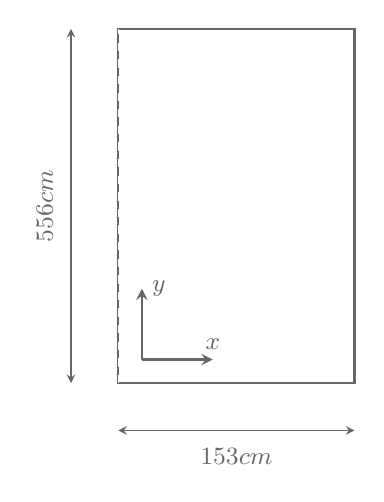
\begin{tikzpicture}[
    scale=1.5,
    cota/.style={<->, >=stealth, thin, gray!80!black},  % Estilo das linhas de cota
    retangulo/.style={draw=gray!80!black, thick},% Estilo do retângulo
    eixo/.style={->, >=stealth, thick, gray!80!black}   % Estilo dos eixos x e y
]

    % 1. Coordenadas do retângulo
    \coordinate (A) at (0, 0);
    \coordinate (B) at (2, 0);
    \coordinate (C) at (2, 3);
    \coordinate (D) at (0, 3);

    % 2. Desenho do Retângulo
    \draw[retangulo] (A) rectangle (C);

    % 3. Eixos de Coordenadas x e y (Origem no canto inferior esquerdo, dentro do retângulo)
    \draw[eixo] (0.2, 0.2) -- (0.8, 0.2) node[above, font=\small\bfseries] {$x$};
    \draw[eixo] (0.2, 0.2) -- (0.2, 0.8) node[right, font=\small\bfseries] {$y$};

    \draw[dashed, white] (A) -- (D);
    
    % --- COTA HORIZONTAL (Texto abaixo da linha) ---
    \def\offsetH{0.4}
    \draw[cota] (0, -\offsetH) -- (2, -\offsetH) 
        node[midway, below=3pt, font=\small] {$153\text{ cm}$};

    % --- COTA VERTICAL (Texto à esquerda da linha) ---
    \def\offsetV{0.4}
    \draw[cota] (-\offsetV, 0) -- (-\offsetV, 3) 
        node[midway, left=3pt, font=\small, rotate=90, anchor=south] {$556 \text{ cm}$};

\end{tikzpicture}
    %\caption{Caption}
    %\label{fig:placeholder}
\end{figure}

        \begin{enumerate}
        \begin{multicols}{2}
            \item Direção horizontal

            $l_0= 150 \ cm$

            $a_1 \leq \begin{cases}
                \frac{b_{w_4}}{2} = 10 \ cm \\
                0,3h = 3 \ cm
            \end{cases}$

            %$a_2 \le \begin{cases}
            %    \frac{b_w}{2} = 00 \ cm \\
            %    0,3 h = 00 \ cm
            %\end{cases}$

            \vspace{2cm}

            $l_{ef}= l_0 +a_1+a_2 = 153 \ cm$
            
            \item Direção vertical

            $l_0= 550\ cm$

            $a_1 \leq \begin{cases}
                \frac{b_{w_2}}{2} = 10 \ cm \\ 
                0,3h = 3 \ cm
            \end{cases}$

            $a_2 \leq \begin{cases}
                \frac{b_{w_3}}{2} = 10 \ cm \\
                0,3 h = 3 \ cm
            \end{cases}$

            $l_{ef}= l_0 +a_1+a_2 = 556 \ cm$
        \end{multicols}

            $\lambda = \frac{l_y}{l_x} = \frac{556}{153} \approx 3,63 > 2 \to$ armada em uma direção
            
        \end{enumerate}

        %\newpage

        \fbox{L4}

        \begin{figure}[H]
    \centering
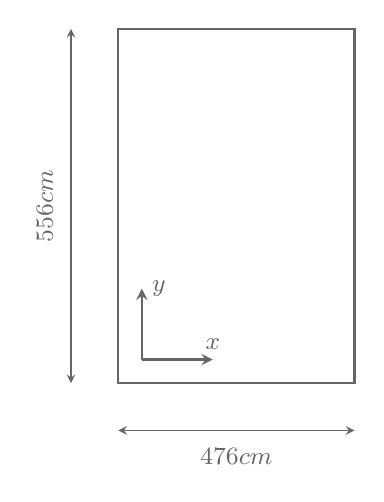
\begin{tikzpicture}[
    scale=1.5,
    cota/.style={<->, >=stealth, thin, gray!80!black},  % Estilo das linhas de cota
    retangulo/.style={draw=gray!80!black, thick},% Estilo do retângulo
    eixo/.style={->, >=stealth, thick, gray!80!black}   % Estilo dos eixos x e y
]

    % 1. Coordenadas do retângulo
    \coordinate (A) at (0, 0);
    \coordinate (B) at (2, 0);
    \coordinate (C) at (2, 3);
    \coordinate (D) at (0, 3);

    % 2. Desenho do Retângulo
    \draw[retangulo] (A) rectangle (C);

    % 3. Eixos de Coordenadas x e y (Origem no canto inferior esquerdo, dentro do retângulo)
    \draw[eixo] (0.2, 0.2) -- (0.8, 0.2) node[above, font=\small\bfseries] {$x$};
    \draw[eixo] (0.2, 0.2) -- (0.2, 0.8) node[right, font=\small\bfseries] {$y$};

    % --- COTA HORIZONTAL (Texto abaixo da linha) ---
    \def\offsetH{0.4}
    \draw[cota] (0, -\offsetH) -- (2, -\offsetH) 
        node[midway, below=3pt, font=\small] {$476\text{ cm}$};

    % --- COTA VERTICAL (Texto à esquerda da linha) ---
    \def\offsetV{0.4}
    \draw[cota] (-\offsetV, 0) -- (-\offsetV, 3) 
        node[midway, left=3pt, font=\small, rotate=90, anchor=south] {$556 \text{ cm}$};

\end{tikzpicture}
    %\caption{Caption}
    %\label{fig:placeholder}
\end{figure}

        \begin{enumerate}
        \begin{multicols}{2}
            \item Direção horizontal

            $l_0= 470 \ cm$

            $a_1 \leq \begin{cases}
                \frac{b_{w_2}}{2} = 10 \ cm \\
                0,3h = 3 \ cm
            \end{cases}$

            $a_2 \leq\begin{cases}
                \frac{b_{w_3}}{2} = 10 \ cm \\
                0,3 h = 3 \ cm
            \end{cases} $

            $l_{ef}= l_0 +a_1+a_2 = 476 \ cm$
            
            \item Direção vertical

            $l_0= 550 \ cm$

            $a_1 \leq \begin{cases}
                \frac{b_{w_4}}{2} = 10 \ cm \\
                0,3h = 3 \ cm
            \end{cases}$

            $a_2 \leq \begin{cases}
                \frac{b_{w_5}}{2} = 10 \ cm \\
                0,3 h = 3 \ cm
            \end{cases}$

            $l_{ef}= l_0 +a_1+a_2 = 556 \ cm$
        \end{multicols}

            $\lambda = \frac{l_y}{l_x} = \frac{556}{476} \approx 1,17 \leq 2 \to$ armada em duas direções
            
        \end{enumerate}
    \end{enumerate}
\end{resposta}